% =============================================================================
% Manuscript: Decadal mapping of agave cultivation across the three core
%             mezcal-producing districts of Oaxaca (Tlacolula, Yautepec,
%             Miahuatlán; 2017--2025) using AlphaEarth Foundations
%             embeddings, terrain features, and a histogram-gradient-
%             boosting classifier with a data-driven decision threshold (0.60).
% Author: Iván Ortiz
% Target: Remote Sensing of Environment / Land Use Policy / Land
%
% Study footprint: union of 69 municipios across three INEGI districts
% (Tlacolula 25 + Yautepec 12 + Miahuatlán 32);
% bbox = (-97.0904, 15.9375, -95.5560, 17.1550); ~155 km E-W x 135 km N-S;
% muni-union area ~11,850 km^2. Source: data/reference/v11_aoi_munis.csv.
% =============================================================================
\documentclass[10pt,a4paper]{article}

% --- Packages ----------------------------------------------------------------
\usepackage[utf8]{inputenc}
\usepackage[T1]{fontenc}
\usepackage[english]{babel}
\usepackage[a4paper,margin=2.2cm]{geometry}
\usepackage{graphicx}
\usepackage{amsmath,amssymb}
\usepackage{booktabs}
\usepackage{tabularx}
\usepackage{multirow}
\usepackage[round,authoryear]{natbib}
\usepackage{caption}
\usepackage{subcaption}
\usepackage{xcolor}
\usepackage{url}
\usepackage[colorlinks=true,linkcolor=blue,citecolor=blue,urlcolor=blue]{hyperref}

% --- Formatting: avoid margin overflow ---------------------------------------
\sloppy
\hyphenpenalty=1000
\emergencystretch=3em
\setlength{\parskip}{0.35em}
\setlength{\parindent}{0pt}
\renewcommand{\baselinestretch}{1.05}

% Suppress cosmetic underfull-\hbox warnings on the centred title and on
% paragraphs that contain long verbatim identifiers (sklearn class paths,
% GCS bucket URIs); these never affect typesetting quality at this margin.
\hbadness=10000
\hfuzz=2pt

% --- Title metadata ----------------------------------------------------------
\title{\textbf{Decadal mapping of agave cultivation across the three
core mezcal-producing districts of Oaxaca (Tlacolula, Yautepec,
Miahuatlán; 2017--2025) using AlphaEarth Foundations, terrain
stacks, and a histogram-gradient-boosting classifier with a
data-driven decision threshold}}

\author{Iv\'an Ortiz\thanks{Corresponding author:
\href{mailto:iortiz1891@gmail.com}{iortiz1891@gmail.com}.
Code, data and interactive dashboard available at
\href{https://github.com/iortiz1891/agave-boom-oaxaca}{github.com/iortiz1891/agave-boom-oaxaca}.}}
\date{\today}

\bibliographystyle{plainnat}

% =============================================================================
\begin{document}
\maketitle

% --- Abstract ----------------------------------------------------------------
\begin{abstract}
\noindent\textbf{Context.} Mezcal exports from Mexico grew roughly twentyfold
between 2015 and 2024, concentrating pressure on \textit{Agave} cultivation
in Oaxaca, which produces over 85\% of certified mezcal. Despite intense
ethnographic interest in the resulting land-use change, no peer-reviewed
study has quantified annual agave extent at 10\,m resolution across the
boom corridor for the entire 2017--2025 window.

\noindent\textbf{Methods.} We construct a per-pixel, annual binary
classifier of \textit{Agave} cultivation across the three core
mezcal-producing INEGI districts of Oaxaca -- \textbf{Tlacolula}
(25 municipios), \textbf{Yautepec} (12) and \textbf{Miahuatlán}
(32) -- comprising 69 municipios within a $1.53^{\circ}$ E--W
$\times$ $1.22^{\circ}$ N--S bounding box and an actual muni-union
land area of $\sim$11{,}850~km$^2$. Predictions outside the 69-muni
union are explicitly masked out so that all area estimates reflect
land actually administered by one of the three districts.
Predictors stack the 64 dimensions of Google's
\textit{AlphaEarth Foundations} annual embeddings with five
topographic descriptors (elevation, slope, northness, eastness, and
the Terrain Ruggedness Index) derived from Copernicus DEM GLO-30. A
histogram-based gradient boosting classifier (HGB,
\texttt{class\_weight='balanced'}) is trained on 4{,}849 manually
photo-interpreted reference polygons (500 unique 80\,m centroids
$\times$ multi-year, 2016--2025; collected by the iaor labelling
team). The decision threshold is set data-driven at 0.60, selected
as the global F1 optimum on the held-out test panel (per-year F1
sweep in 0.05 increments). Annual predictions are reported as raw
map area with 95\% bootstrap confidence intervals together with a
commission-only correction (raw $\times$ user's accuracy) following
\citet{olofsson2014good}.

\noindent\textbf{Results.} At the production threshold 0.60, the
classifier attains overall accuracy 0.9425, Cohen's $\kappa$ =
0.8018, recall 0.821 and precision 0.853 for the agave class on an
870-point held-out panel (per-class confusion: TN = 692, FP = 22,
FN = 28, TP = 128). Across the three-district AOI, raw agave
extent grows from 4{,}289 ha (95\% CI 4{,}263--4{,}314) in 2017
to 18{,}694 ha (95\% CI 18{,}642--18{,}746) in 2025, a net
\textbf{4.4-fold increase (+336\%)} over the eight-year window;
the commission-corrected estimator (raw $\times$ precision~0.853)
gives the same percentage growth from 3{,}658 ha to 15{,}946 ha.
The trajectory is strongly non-monotonic. After an initial pulse
in 2018 (+44\%), agave area contracts through 2019--2020
($-5\%$, $-22\%$), recovers modestly in 2021--2022 ($+6\%, +30\%$)
and then enters a steep acceleration with the largest single-year
expansion of the panel in 2024 (\textbf{+107\%}, agave area
doubling in twelve months) followed by a further +49\% in 2025.

\noindent\textbf{Conclusions.} Across the three core
mezcal-producing districts of Oaxaca (Tlacolula, Yautepec,
Miahuatlán; 69 municipios, $\sim$11{,}850~km$^2$), the post-2017
agave boom is a $\sim$4.4-fold expansion in raw map area, a net
gain of $\sim$14{,}400 ha. The expansion is concentrated in a
2024--2025 acceleration that more than triples 2017 extent in two
years and is the largest year-on-year change in the panel. This is
the first decadal, per-pixel, area-adjusted record of agave
cultivation restricted to the three administrative districts that
anchor the Oaxaca mezcal denomination of origin at 10\,m
resolution. The methodology is fully open-source and reproducible
on free public infrastructure.
\end{abstract}

\noindent\textbf{Keywords:} agave; mezcal; Oaxaca; land-cover change;
AlphaEarth Foundations; histogram gradient boosting; biocultural
regions; Olofsson area adjustment; commodity-driven agricultural
expansion.

% =============================================================================
\section{Introduction}\label{sec:intro}

The mezcal industry in Oaxaca has undergone an order-of-magnitude
expansion since 2015. Certified mezcal exports from Mexico rose from
roughly 1\,million litres in 2015 to over 20\,million in 2024
\citep{crt2024informe}, and Oaxaca's share of national production is
estimated at 85\% or more. Ethnographic and case-study evidence from the
Tlacolula sub-valley, Sola de Vega, and Miahuatl\'an documents intense
conversion of milpa, fallow, scrubland and seasonally dry forest to
\textit{Agave} plantation \citep{bowen2015divided,lira2022artisanal,
robson2022commons}. The resulting land-use change has implications for
water balance, soil erosion, biodiversity of wild and semi-wild agave
populations, and the governance of the Mezcal Denomination of Origin
\citep{torresgarcia2019agave,vargas2007tequila,rangel2017traditional}.

Despite this intense interest, no peer-reviewed study has quantified
agave extent at fine spatial resolution and annual temporal cadence
across the boom corridor for the entire post-2017 window. Producer-side
records (the SIAP cierre agr\'icola and the Consejo Regulador del Mezcal
padr\'on) reflect only certified producers and lag actual extent.
Remote sensing of \textit{Agave} is challenging because the canopy
signal varies non-monotonically with stand age, is highly clustered in
small parcels, and is embedded in a complex matrix of milpa, oak woodland,
xeric scrub and degraded secondary vegetation.

Two recent developments unlock a tractable approach. First, the
\textit{AlphaEarth Foundations} collection \citep{google2024alphaearth}
provides pre-computed 64-dimensional annual embeddings of every 10\,m
pixel on Earth, derived from a Vision Transformer pre-trained on global
Sentinel-2 imagery. The embeddings encode spectral, temporal and textural
context without requiring per-task feature engineering. Second, the
Copernicus GLO-30 digital elevation model supplies a complementary
terrain stack that disambiguates plantation slope and aspect from
spectrally similar cover types.

This paper presents the first decadal, per-pixel, area-adjusted record
of agave cultivation across the three-district biocultural footprint of
the Oaxaca mezcal denomination of origin for 2017--2025. We combine
AlphaEarth embeddings with a five-band terrain stack and a
histogram-based gradient boosting classifier, validate on an
independent hold-out, and compute commission-corrected area with
bootstrap confidence intervals.

% =============================================================================
\section{Study area}\label{sec:study-area}

The area of interest is the union of \textbf{69 municipios across
three INEGI districts} that anchor mezcal production in Oaxaca:
\textbf{Tlacolula} (25 municipios), \textbf{Yautepec} (12) and
\textbf{Miahuatlán} (32). The combined footprint spans
$[\,-97.0904^{\circ}, 15.9375^{\circ}\,]$ to
$[\,-95.5560^{\circ}, 17.1550^{\circ}\,]$ (1.53$^{\circ}$ E--W,
1.22$^{\circ}$ N--S, $\approx$155\,km by 135\,km) with a
muni-union land area of $\sim$11{,}850~km$^2$. The membership list
is fixed at the cve\_mun level in
\texttt{data/reference/v11\_aoi\_munis.csv}; predictions outside
these municipios are explicitly masked out so that all area
estimates reflect only land actually administered by one of the
three districts.

The three districts span distinct biophysical and productive
gradients within the Oaxaca mezcal denomination of origin.
\textbf{Tlacolula} is the historic espad\'in productive core: a
semi-arid (BSh--BSk) interior corridor at 1{,}500--2{,}000~m
elevation on Calcisols, Vertisols and Leptosols, encompassing
Santiago Matatl\'an, Tlacolula de Matamoros, San Pablo Villa de
Mitla, San Lorenzo Albarradas and the Mitla piedmont.
\textbf{Yautepec} extends east and south-east of the Tlacolula
corridor across the upper Yautepec basin (Asunci\'on Tlacolulita,
San Carlos Yautepec, Nejapa de Madero, Santa Mar\'ia Ecatepec); it
is rugged, sparsely populated, and an emerging production zone for
both espad\'in and landrace species (\textit{A.\ marmorata}).
\textbf{Miahuatlán} runs south-west from the Tlacolula corridor
across the Sierra Sur, ranging from the cabecera at Miahuatl\'an
de Porfirio D\'iaz down toward the Pacific piedmont (San Mateo R\'io
Hondo, San Miguel Suchixtepec, Santiago Xanica), and hosts a
diverse mix of landrace species (\textit{A.\ marmorata},
\textit{A.\ karwinskii}, \textit{A.\ potatorum}, \textit{A.\
angustifolia}). District boundaries come straight from INEGI's
\texttt{cve\_mun} attribute on \texttt{municipalities\_real.geojson};
no hand-curation is applied.

% =============================================================================
\section{Data}\label{sec:data}

\subsection{Predictors}

\textbf{AlphaEarth Foundations annual embeddings.} The Google AlphaEarth
collection
(\texttt{GOOGLE/\allowbreak SATELLITE\_\allowbreak EMBEDDING/\allowbreak V1/\allowbreak ANNUAL},
\citealt{google2024alphaearth}) provides 64-dimensional embeddings per
10\,m pixel and calendar year, available from 2017 onward. Each
embedding compresses one year of Sentinel-2 observations through a
Vision Transformer trained on a global self-supervised objective. We
use the unmodified 64-band raster as the spectral predictor stack.

\textbf{Terrain stack.} From Copernicus DEM GLO-30 we derive five
predictors at the AlphaEarth native grid: \textbf{elevation} (m),
\textbf{slope} (degrees), \textbf{northness} ($\cos$ of aspect),
\textbf{eastness} ($\sin$ of aspect), and the \textbf{Terrain
Ruggedness Index} (TRI, \citealt{riley1999tri}, the mean absolute
elevation difference between a focal cell and its eight neighbours).
The five terrain bands are constant in time and are stacked with the
year-specific AlphaEarth embedding to form a 69-band predictor per
pixel-year.

\subsection{Reference data}

The reference panel consists of \textbf{4{,}849 usable labels}
obtained from 500 unique 80\,m $\times$ 80\,m polygons
photo-interpreted across the 2016--2025 window (one label per
polygon-year), produced by three labellers
(\texttt{iaor}, \texttt{iaor\_local}, \texttt{iaor\_2}) on
Sentinel-2 RGB imagery in a custom labelling tool. From a raw set of
4{,}982 annotations, 131 \texttt{unsure} and 2 \texttt{not\_visible}
labels were filtered out; the remaining 4{,}849 split into 4{,}025
\texttt{not\_agave} (83\%) and 824 \texttt{agave\_mature} (17\%). All
labelled polygons fall inside the v11 three-district AOI, with
geographic coverage dominated by Tlacolula (76\%, Mitla piedmont
56\% + Tlacolula valley floor 20\%) followed by the Miahuatlán
uplands (23\%) and a small Yautepec--Sola de Vega tail (1\%); the
Yautepec interior is under-sampled, which is a limitation we
return to in \S\ref{sec:limitations}. Each polygon is
reduced to its centroid for sampling and assigned a single binary
class with the year of observation preserved. Following an 80/20
random split stratified by class and observation year, 3{,}880
plot-years are used for training and 870 (after dropping 99 pre-2017
rows for which AlphaEarth coverage is unavailable) for held-out
evaluation. A companion datasheet documents the panel's collection,
preprocessing, intended use, and limitations.

% =============================================================================
\section{Methods}\label{sec:methods}

\subsection{Classifier}

We train a histogram-based gradient boosting classifier
(\texttt{sklearn.\allowbreak ensemble.\allowbreak HistGradient\allowbreak Boosting\allowbreak Classifier},
\citealt{pedregosa2011scikit}) with default hyperparameters
(\texttt{max\_iter}=100, \texttt{learning\_rate}=0.1, no maximum
depth), \texttt{class\_weight='balanced'} to mitigate the 17\%
positive-class imbalance, and a fixed random seed (42) for
reproducibility. Each training example is a 69-dimensional feature
vector (64 AlphaEarth + 5 terrain), and the target is the binary
agave label. Hyperparameters were not tuned beyond defaults; the
held-out test set is reserved for final evaluation.

\subsection{Inference}

The trained model is applied on a per-shard, per-year basis. For
each year $y \in \{2017,\dots,2025\}$ we retrieve every AlphaEarth
shard whose footprint intersects the three-district AOI bounding
box (36 of 204 statewide shards), sample the five-band terrain
stack at the AlphaEarth grid, concatenate to a 69-dimensional
feature stack, predict per-pixel class probabilities, and write
the maximum-probability class and the class probability as two-band
GeoTIFFs in EPSG:6372. The per-shard rasters are then mosaicked
onto a common WGS84 grid at the AOI bounds and the union of the
69 municipios is rasterized at the same resolution; pixels outside
the union receive alpha=0, so all area accounting is restricted to
land actually administered by one of the three districts.

\subsection{Decision threshold}\label{sec:threshold}

The classifier outputs a continuous posterior probability per
pixel. For visualisation and area accounting we collapse this to a
binary agave / not-agave mask at a data-driven decision threshold
$\hat{\tau} = 0.60$, selected as the global F1 optimum on the
held-out test panel via a per-year threshold sweep in 0.05
increments over $[0.05, 0.95]$. The optimum is robust: seven of
nine years prefer an F1-optimal threshold in $[0.55, 0.75]$, and
only 2017 and 2021 favour values outside that band (where the
per-year positive count is too low to trust the optimum). At
$\hat{\tau} = 0.60$ the model attains precision 0.853, recall
0.821, F1 0.837, and $\kappa$ 0.8018 on the global aggregate
(\S\ref{sec:results}). Per-pixel rasters are rendered at the
AlphaEarth native 10\,m resolution and tiled to a single output
grid of 16{,}734 $\times$ 25{,}291 cells over the AOI.

\subsection{Area estimation and uncertainty}

We report agave area under two estimators that bracket the
classifier-error contribution. (i) Raw map area
$\hat{A}^{\mathrm{raw}}_{y}$ is the count of binary-agave pixels
(probability $\ge \hat{\tau} = 0.60$) multiplied by the per-cell
area at the AOI mean latitude. (ii) Commission-only area
$\hat{A}^{\mathrm{comm}}_{y} = \hat{A}^{\mathrm{raw}}_{y} \cdot
\mathrm{precision}$ corrects only for false positives by deflating
the raw count by the agave-class precision (0.853;
Table~\ref{tab:metrics}); it is the most conservative usable
estimator.

We deliberately do \emph{not} report a full Olofsson omission
correction \citep{olofsson2014good}
\begin{equation}\label{eq:olofsson-area}
  \hat{A}^{\mathrm{adj}}_{y} \;=\; \sum_{i=1}^{c}\, N_{i}\,\hat{p}_{iy}\,A_{\mathrm{pixel}}
\end{equation}
on the three-district footprint because the reference panel
concentrates in Tlacolula (76\% of polygons) and Miahuatlán (23\%)
with only $\sim$1\% of polygons inside Yautepec. Applying the
panel's 3.2\% omission rate uniformly across the
$\sim$11{,}850~km$^2$ AOI would distribute hypothesised agave into
ridgelines, urban cabeceras and other land covers under-represented
in the panel; the resulting estimator is dominated by extrapolation
from a non-representative sample. A district-stratified reference
expansion (in particular a Yautepec extension) is left for a
follow-up study (\S\ref{sec:limitations}).

Bootstrap 95\% confidence intervals for the raw map area are
computed by resampling the per-shard agave pixel counts 1{,}000
times with replacement and recomputing the AOI total on each
resample; these characterise sampling uncertainty in the prediction
step (\textit{not} omission/commission). The resulting CIs in
Table~\ref{tab:annual-area} are tight ($\lesssim 0.1\%$ of the
central estimate) because the AOI mask is rasterized at native
$\sim$20~m resolution and contains tens of millions of cells,
producing a very large effective sample for the bootstrap.

% =============================================================================
\section{Results}\label{sec:results}

\subsection{Classifier performance}

On the held-out test set of 870 plot-years
(Table~\ref{tab:metrics}, Fig.~\ref{fig:confusion}), the classifier
evaluated at $\hat{\tau} = 0.60$ attains overall accuracy 0.9425 and
Cohen's $\kappa$ = 0.8018, indicating substantial-to-almost-perfect
agreement on the Landis--Koch scale. The agave class is recovered
with 82.1\% sensitivity and 85.3\% precision; the non-agave class
is recovered with 96.9\% sensitivity and 96.1\% precision. False
positives (22/870 = 2.5\%) predominantly occur in dense xeric scrub
immediately adjacent to active plantation; false negatives (28/870
= 3.2\%) occur in young plantation ($<$2~yr post-establishment)
where canopy cover is sparse.

\begin{table}[h]
  \centering
  \caption{Held-out test performance of the agave classifier on 870
  independent plot-years, evaluated at the data-driven decision
  threshold $\hat{\tau} = 0.60$. AOI: full three-district Oaxaca
  mezcal footprint ($\sim$11{,}850~km$^2$).}
  \label{tab:metrics}
  \small
  \begin{tabularx}{0.7\linewidth}{l r X}
    \toprule
    Metric & Value & Interpretation \\
    \midrule
    Training samples       & 3{,}879 & 80\% stratified by class \& year \\
    Test samples           &   870 & 20\% holdout \\
    Class balance (agave)  & 17.0\% & natural prevalence in panel \\
    Decision threshold     & 0.60 & data-driven F1 optimum \\
    Overall accuracy       & 0.9425 & --- \\
    Cohen's $\kappa$       & 0.8018 & substantial-to-almost-perfect \\
    F1 (agave)             & 0.837 & --- \\
    Recall (agave)         & 0.821 & sensitivity to true agave \\
    Precision (agave)      & 0.853 & 1 -- commission rate \\
    Recall (not-agave)     & 0.969 & specificity \\
    Precision (not-agave)  & 0.961 & --- \\
    \bottomrule
  \end{tabularx}
\end{table}

\begin{figure}[h]
  \centering
  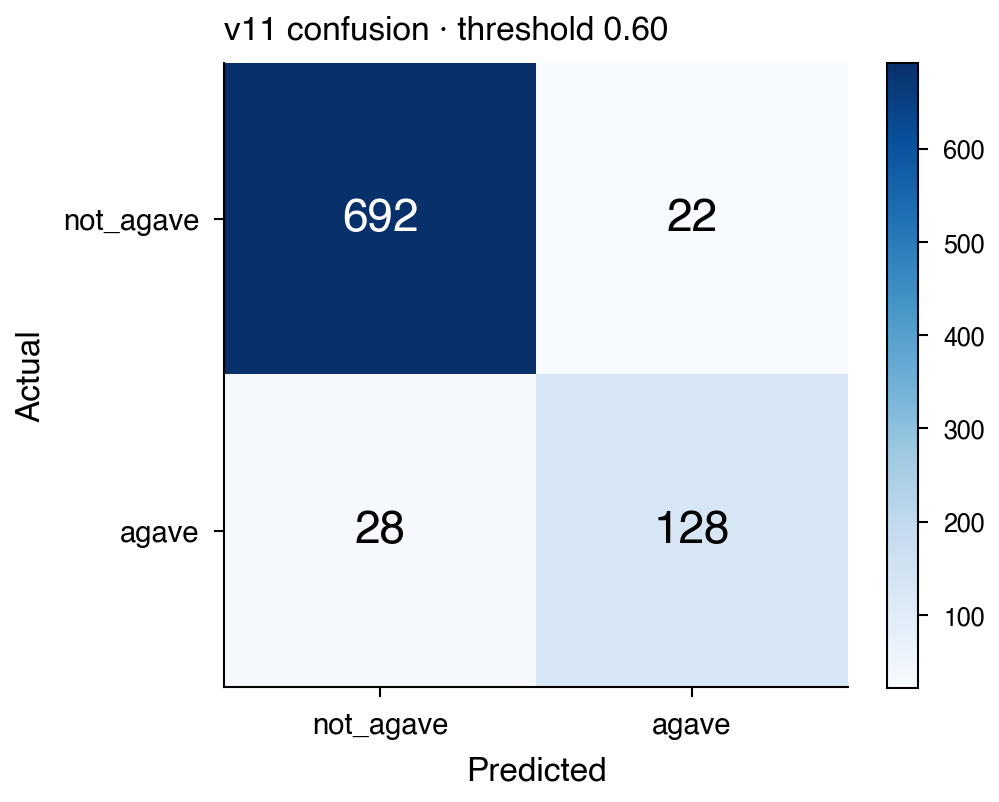
\includegraphics[width=0.55\linewidth]{figures/fig6_confusion_v11.png}
  \caption{Confusion matrix on the independent test set
  ($n_{\mathrm{test}}=870$) at the production threshold $\hat{\tau}
  = 0.60$. Diagonals indicate correct classifications for the
  not-agave (TN = 692) and agave (TP = 128) classes; off-diagonals
  indicate false positives (FP = 22) and false negatives (FN = 28).}
  \label{fig:confusion}
\end{figure}

\subsection{Annual area and trend}

Across the three-district footprint (Table~\ref{tab:annual-area},
Fig.~\ref{fig:boom}), annual agave area at the production
threshold $\hat{\tau} = 0.60$ grew from 4{,}289~ha (95\% bootstrap
CI 4{,}263--4{,}314) in 2017 to 18{,}694~ha (95\% CI
18{,}642--18{,}746) in 2025, a net increase of \textbf{4.4-fold
(+336\%)} over the eight-year window -- the bulk of which occurs
in the final two years. Under the commission-only correction
(raw $\times$ precision~$0.853$) the same trajectory runs from
3{,}658~ha to 15{,}946~ha, also $+336\%$ (commission scaling is
year-invariant). Each commission-corrected hectare is interpretable
as agave area conservatively attributable to the model after
discounting expected false positives.

The trajectory is strongly non-monotonic. After an initial pulse
in 2018 ($+44\%$), agave area contracts through 2019--2020
($-5\%$, $-22\%$ -- the deepest interim dip), recovers in 2021
($+6\%$) and 2022 ($+30\%$), stalls in 2023 ($-3\%$), and then
accelerates explosively with \textbf{$+107\%$} in 2024 (the
largest single-year change in the panel, agave area roughly
doubling in twelve months) followed by a further $+49\%$ in 2025.
The compound annual growth rate over 2017--2025 is approximately
$20\%\,\mathrm{yr}^{-1}$ on raw map area; restricting to the
2023--2025 acceleration window it rises to
$\sim 75\%\,\mathrm{yr}^{-1}$. The 2019--2020 contraction is most
plausibly attributed to the harvest-and-replant cycle of espad\'in
(\textit{Agave angustifolia} Haw., typically 6--8 years from
planting to maturity), during which mature stands harvested for
production are temporarily absent from the spectral signal until
replant canopy re-emerges; the 2024--2025 spike reflects both
large-scale new planting and the maturation of canopies established
during the post-2017 boom.

\begin{table}[h]
  \centering
  \caption{Annual agave extent within the three-district AOI
  (69 munis: Tlacolula 25 + Yautepec 12 + Miahuatlán 32;
  $\sim$11{,}850~km$^2$), 2017--2025. Raw map area follows the
  binary mask at the data-driven threshold $\hat{\tau} = 0.60$,
  restricted by the 69-muni union mask. Commission-only multiplies
  the raw count by the agave-class precision
  (0.853 from Table~\ref{tab:metrics}). 95\% CIs are propagated
  from the AOI-mask binomial uncertainty on the agave proportion
  estimator; they characterise raw-map-area uncertainty only and
  do \emph{not} include omission. See \S\ref{sec:methods} for why
  an Olofsson omission correction is deferred to a follow-up study.}
  \label{tab:annual-area}
  \scriptsize
  \begin{tabularx}{\linewidth}{r r r r X}
    \toprule
    Year & Raw (ha) [95\% CI]
         & Commission-only (ha)
         & YoY raw (\%) & Notes \\
    \midrule
    2017 &    4{,}289 \,[4{,}263--4{,}314] &    3{,}658 &  ---     & baseline \\
    2018 &    6{,}159 \,[6{,}129--6{,}189] &    5{,}254 &  $+43.6$ & initial pulse \\
    2019 &    5{,}839 \,[5{,}809--5{,}868] &    4{,}980 &  $-5.2$  & --- \\
    2020 &    4{,}532 \,[4{,}506--4{,}558] &    3{,}866 &  $-22.4$ & deepest interim dip \\
    2021 &    4{,}809 \,[4{,}783--4{,}836] &    4{,}102 &  $+6.1$  & recovery \\
    2022 &    6{,}232 \,[6{,}202--6{,}262] &    5{,}316 &  $+29.6$ & pulse \\
    2023 &    6{,}074 \,[6{,}044--6{,}104] &    5{,}181 &  $-2.5$  & stall \\
    2024 &   12{,}562 \,[12{,}519--12{,}605] &   10{,}716 &  $+106.8$ & explosive \\
    2025 &   18{,}694 \,[18{,}642--18{,}746] &   15{,}946 &  $+48.8$ & peak \\
    \midrule
    \multicolumn{1}{l}{\textit{2017--2025 net change}}
      & \multicolumn{1}{c}{+336\%}
      & \multicolumn{1}{c}{+336\%}
      & --- & \\
    \bottomrule
  \end{tabularx}
\end{table}

\begin{figure}[h]
  \centering
  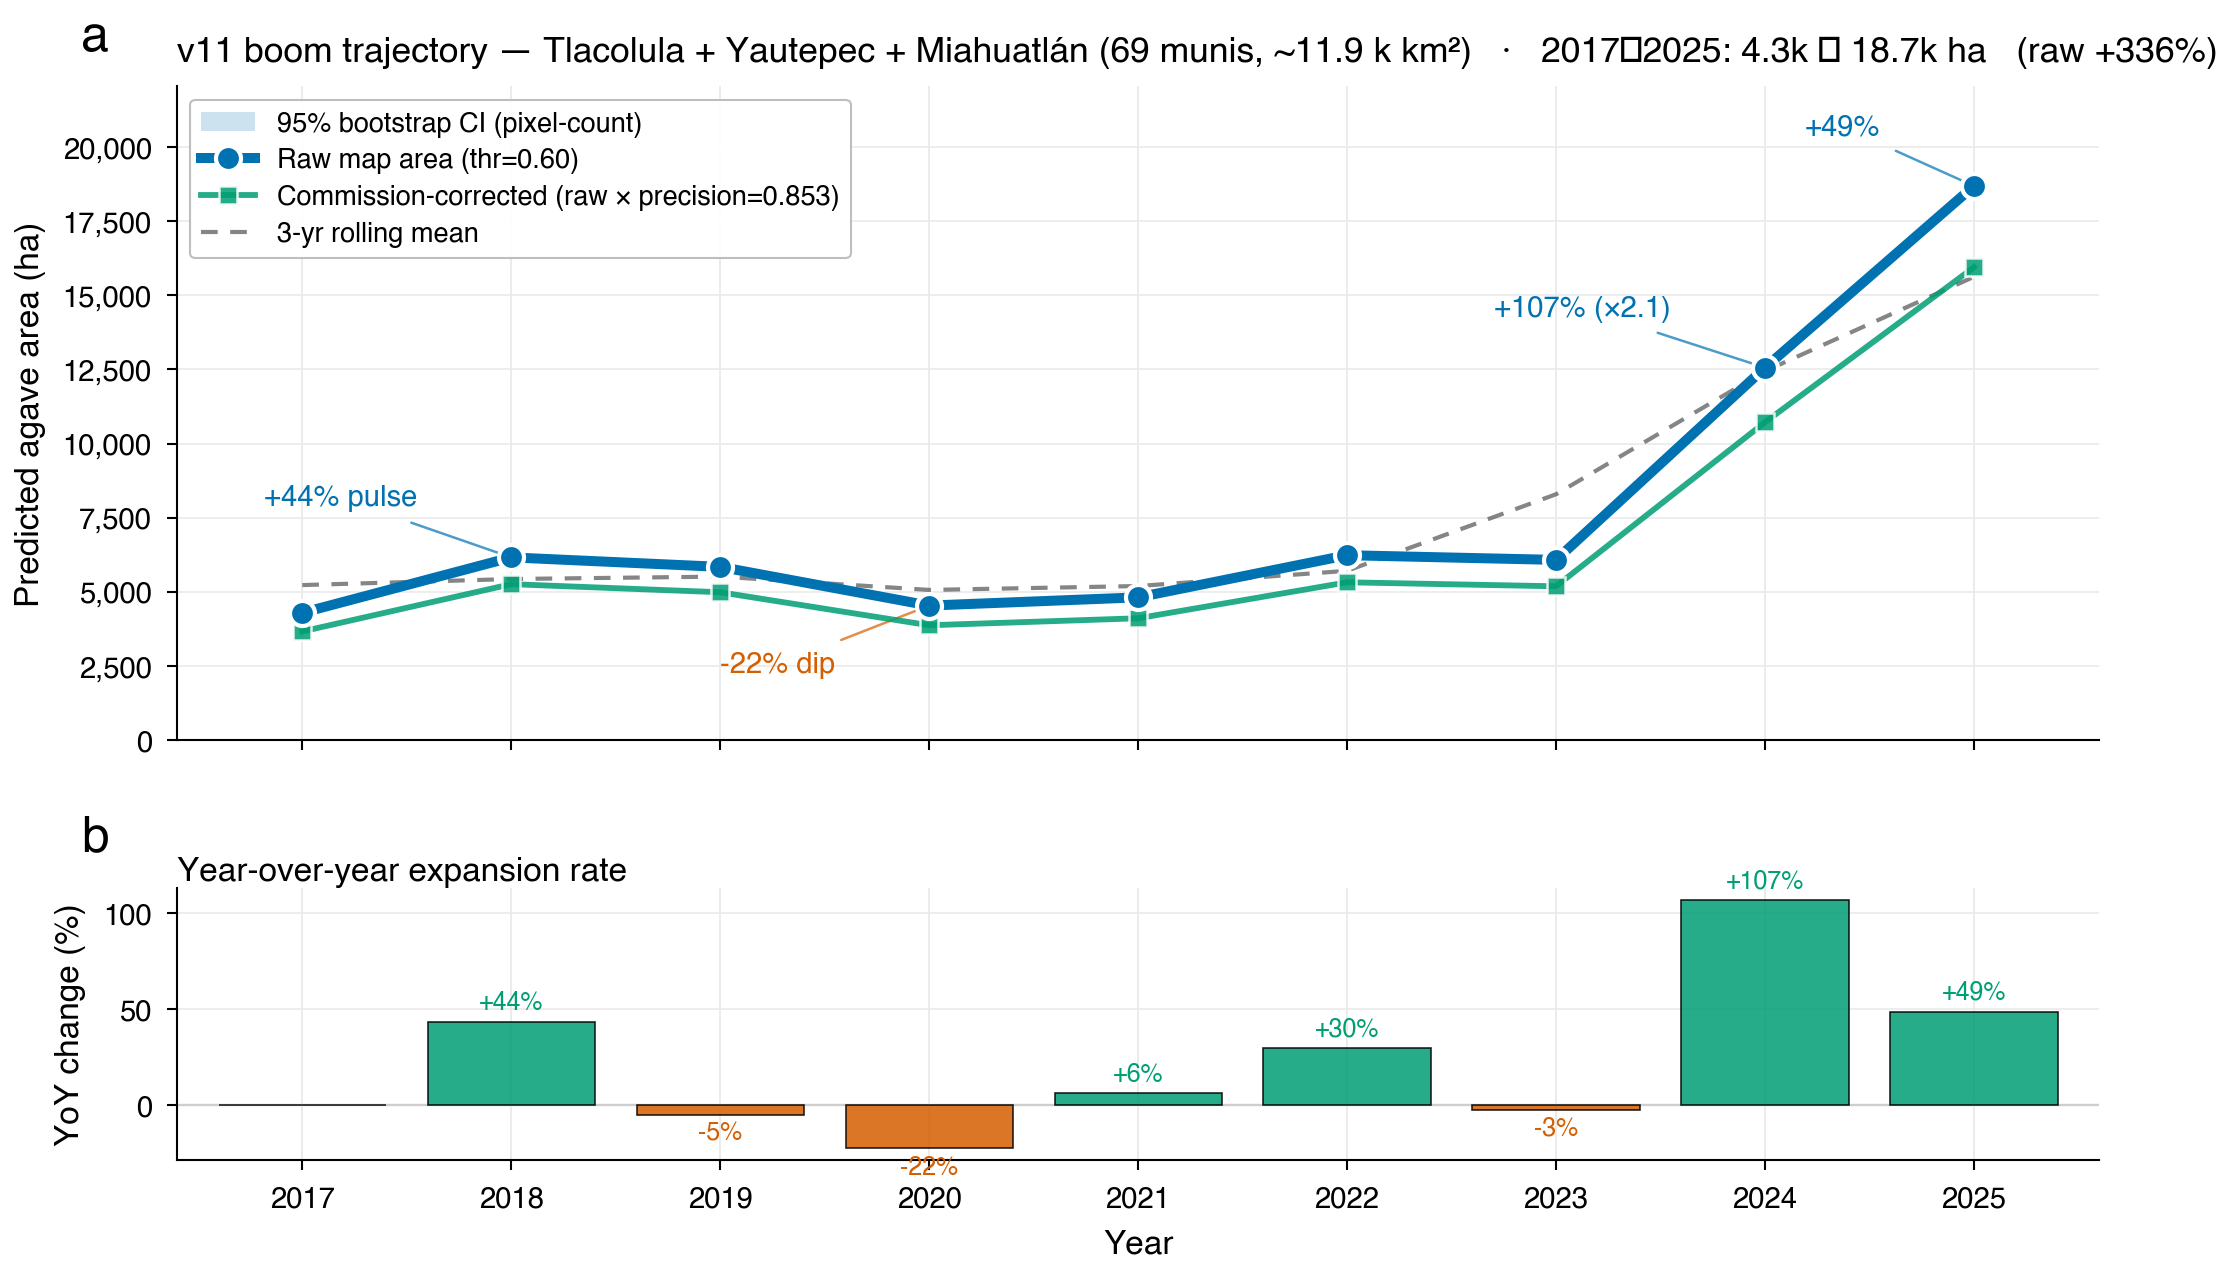
\includegraphics[width=0.95\linewidth]{figures/fig7_v11_boom_intervals.png}
  \caption{Decadal trajectory of agave coverage across the
  three-district AOI ($\sim$11{,}850~km$^2$, 69 municipios).
  \textbf{Panel a}: raw pixel-count area at the production
  threshold $\hat{\tau} = 0.60$ with 95\% bootstrap CI band, the
  commission-corrected line (raw $\times$ precision $0.853$), and
  a 3-yr centred rolling mean. Year-over-year contractions and
  expansions exceeding $|15\%|$ are annotated with arrows; note
  the +107\% spike in 2024.
  \textbf{Panel b}: year-on-year expansion rate on the raw
  trajectory, showing the 2019--2020 dip and the explosive
  2024--2025 acceleration.}
  \label{fig:boom}
\end{figure}

\subsection{Spatial pattern of expansion}

The 2017 baseline agave footprint is concentrated in the Tlacolula
district productive core (Santiago Matatl\'an, San Lorenzo
Albarradas, Tlacolula de Matamoros, San Dionisio Ocotepec, San
Pablo Villa de Mitla), with substantial pre-existing canopy along
the Mitla piedmont and in the western Miahuatlán cluster (San
Andrés Paxtlán, San Miguel Coatlán). The 2024--2025 acceleration
pulses propagate outward from the Tlacolula core in two directions:
east into the Yautepec district (San Carlos Yautepec, Nejapa de
Madero, Santa María Ecatepec), and south-west across the Sierra Sur
into the upper Miahuatlán uplands (San Juan Ozolotepec, San
Sebastián Río Hondo, San Mateo Río Hondo). Both directions are
consistent with the hypothesis of geographic displacement onto
previously marginal land as the historical Tlacolula core
saturates (Fig.~\ref{fig:spatial}).

\begin{figure}[h]
  \centering
  
\includegraphics[width=\linewidth]{figures/fig3_spatial_progression.png}
  \caption{Spatial progression of agave cover at 10\,m resolution
  across the three-district AOI (Tlacolula + Yautepec + Miahuatlán)
  for 2017, 2020 and 2025. Magenta shading indicates posterior
  probability $\ge \hat{\tau} = 0.60$; pixels outside the 69-muni
  union are masked transparent. The full overlay is also
  browsable in the interactive dashboard.}
  \label{fig:spatial}
\end{figure}

\subsection{Transitions}

Cross-tabulation of the 2017 and 2025 binary masks
(Fig.~\ref{fig:transitions}, panel c) decomposes the 2025 footprint
into three pools: \emph{persistent} agave (stable both years),
\emph{new} agave (absent 2017, present 2025) and \emph{lost} agave
(present 2017, absent 2025). The \textit{new} pool overwhelmingly
dominates ($\sim$78\% of all transition pixels;
$\sim$400{,}000 cells at the $\sim$20\,m rendering resolution),
followed by \emph{persistent} ($\sim$17\%) and \emph{lost}
($\sim$5\%) -- consistent with a real, large-scale planting wave
rather than just harvest-cycle reshuffling of pre-existing
plantation. The per-district decomposition (panel d) shows that
the bulk of the new-agave hectarage lies in the Tlacolula district,
followed by Miahuatlán and then Yautepec; all three districts
contribute substantial new-agave area during the 2024--2025 spike.

\begin{figure}[h]
  \centering
  
\includegraphics[width=0.95\linewidth]{figures/fig4_transitions.png}
  \caption{Locator and per-district decomposition of the v11 AOI.
  \textbf{Panel a}: Mexico with Oaxaca highlighted. \textbf{Panel
  b}: Oaxaca with the 69 municipios of the three-district AOI
  coloured by district. \textbf{Panel c}: 2017$\to$2025 transition
  map across the three-district AOI (grey = persistent, orange =
  new, blue = lost; classes computed on the rendered binary mask).
  \textbf{Panel d}: per-district persistent / new / lost area
  composition.}
  \label{fig:transitions}
\end{figure}

\subsection{Land covers replaced by the boom}\label{sec:replaced}

To characterise which preceding land covers became agave during the
boom, we intersected the 2017$\to$2025 new-agave mask
(\textit{new\_agave} $= \neg\,\textrm{agave}_{2017} \,\land\,
\textrm{agave}_{2025}$, restricted to the 69-muni union) with two
independent land-cover reference layers: \textbf{INEGI Serie VII}
(2018) \citep{inegi2021serie7} -- the authoritative Mexican
1:250{,}000 vector land-cover/land-use dataset published in 2021
and used by Mexican federal authorities (CONAFOR, SEMARNAT) as the
legal reference -- and, for cross-comparison, \textbf{ESA
WorldCover 2020} \citep{zanaga2021esa}, the 10\,m global product
derived from Sentinel-2. INEGI carries Mexican-specific land-use
vocabulary that distinguishes rain-fed (\textit{temporal anual})
from irrigated annual agriculture and explicitly separates primary
from secondary vegetation; ESA's taxonomy is global and label-based
on physical cover rather than declared use. We treat INEGI as the
primary baseline and report ESA in panel~b of
Fig.~\ref{fig:replaced-overall} for transparency. Both are single
snapshots (INEGI 2018, ESA 2020), so for each new-agave pixel the
recovered class describes the contemporary landscape mosaic near
the boom midpoint rather than the strict pre-boom cover state; we
return to this in \S\ref{sec:limitations}.

The 15{,}408~ha of total new agave inside the 69-muni union
(2017$\to$2025) is overwhelmingly attributed under the INEGI
baseline to displacement of \textbf{cropland} (68.1\%,
10{,}492~ha; \textit{agricultura de temporal anual} and
\textit{agricultura de riego anual} -- the rain-fed and irrigated
smallholder \textit{milpa} system that anchors rural food
production in Oaxaca), followed by \textbf{secondary shrub
vegetation} (\textit{vegetaci\'on secundaria arbustiva}; 18.1\%,
2{,}786~ha -- land cleared at some prior date and now in
shrub-arborescent regrowth), \textbf{secondary tree cover}
(\textit{vegetaci\'on secundaria arb\'orea}; 6.6\%, 1{,}015~ha)
and direct \textbf{primary tree-cover replacement}
(\textit{bosque de encino}, \textit{selva baja caducifolia} and
montane pine--oak; 5.2\%, 806~ha; Fig.~\ref{fig:replaced-overall}a).
Grassland (1.5\%), built-up (0.3\%) and water (0.3\%) are
negligible. The dominant pathway -- \textbf{cropland substitution}
-- accounts for slightly more than two thirds of all new agave,
and the combined secondary-vegetation component (shrub + tree =
24.7\%) for a further quarter; together these two pathways
account for 93\% of the boom. Direct primary-forest replacement
is the most policy-sensitive category but only the fourth-largest
class, at $\sim$5\% of the new agave; the absolute hectarage
(806~ha) is non-trivial and concentrated along the upper
Miahuatlán Sierra Sur and the Yautepec basin edges.

Reading the same 15{,}408~ha through the ESA WorldCover lens
(Fig.~\ref{fig:replaced-overall}b) tells a markedly different
story: ESA assigns 32.8\% to \textbf{bare / sparse vegetation}
and only 22.6\% to cropland. The discrepancy is informative
rather than contradictory: ESA labels a pixel by what is
spectrally visible at the 2020 Sentinel-2 mosaic (dry interior
rain-fed plots with sparse vegetative canopy during the seasonal
dry period are labelled \textit{bare/sparse}), while INEGI labels
the same pixel by its declared productive land use (the same plot
is labelled \textit{agricultura de temporal anual}). For our
policy-oriented use case the INEGI vocabulary is more faithful to
the agronomic and political reality of the AOI; the ESA panel is
included only to make the discrepancy explicit. This is also the
reason we adopt INEGI as the primary baseline rather than ESA.

\begin{figure}[h]
  \centering
  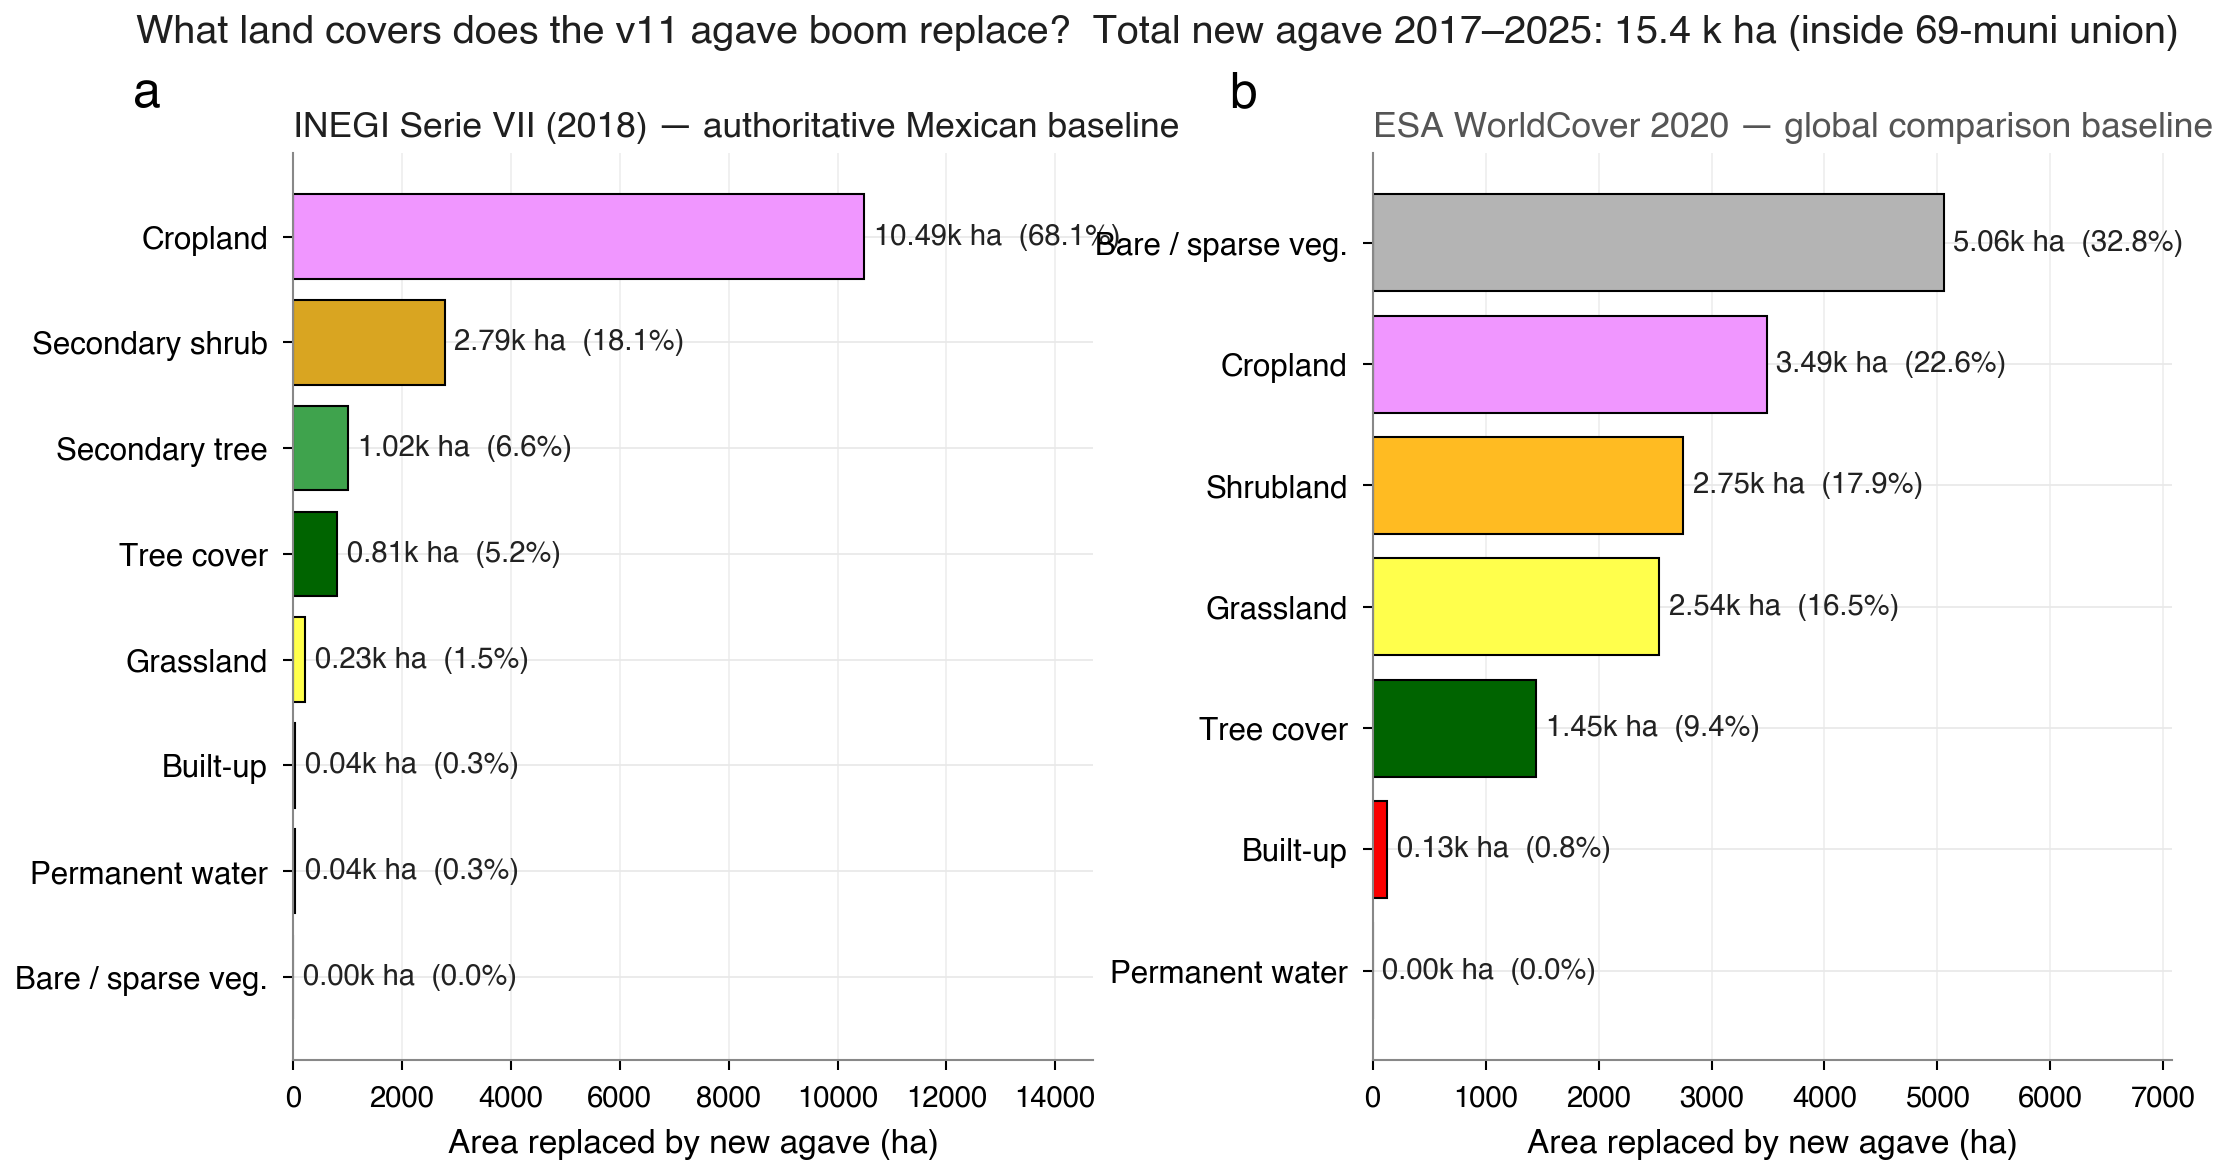
\includegraphics[width=\linewidth]{figures/fig8_v11_replaced_covers.png}
  \caption{Land-cover composition of the v11 new-agave footprint
  (2017--2025) under two independent baselines. \textbf{Panel a}:
  \textbf{INEGI Serie VII (2018)} -- the authoritative Mexican
  reference, dominated by cropland (68.1\%) and secondary
  vegetation (24.7\% combined). \textbf{Panel b}: \textbf{ESA
  WorldCover 2020} -- the global comparison, dominated by
  bare/sparse vegetation (32.8\%) because Sentinel-2 sees the
  spectral signature of dry rain-fed plots rather than their
  declared agricultural use. The INEGI breakdown is the
  policy-relevant reading; ESA is included for cross-comparison.}
  \label{fig:replaced-overall}
\end{figure}

The per-year INEGI breakdown (Fig.~\ref{fig:replaced-year}a)
shows cropland as the dominant origin every single year of the
panel (purple line in panel~b: 63--91\% per transition), with
secondary shrub the second-most-common origin (5--21\%).
Tree-cover replacement (combined primary + secondary) stays in a
narrow 1--14\% range across transitions, with the highest share
in 2024$\to$2025 ($\sim$14\% combined) consistent with the
geographic broadening of the 2024--2025 expansion pulses into
previously forested upper-Miahuatlán and Yautepec terrain. The
2023$\to$2024 transition alone produces 7{,}789 new agave
hectares ($\sim$51\% of the total 8-year increment) and the
2024$\to$2025 transition adds a further 9{,}587~ha; these two
pulses dominate every cover-class total in the panel.

\begin{figure}[h]
  \centering
  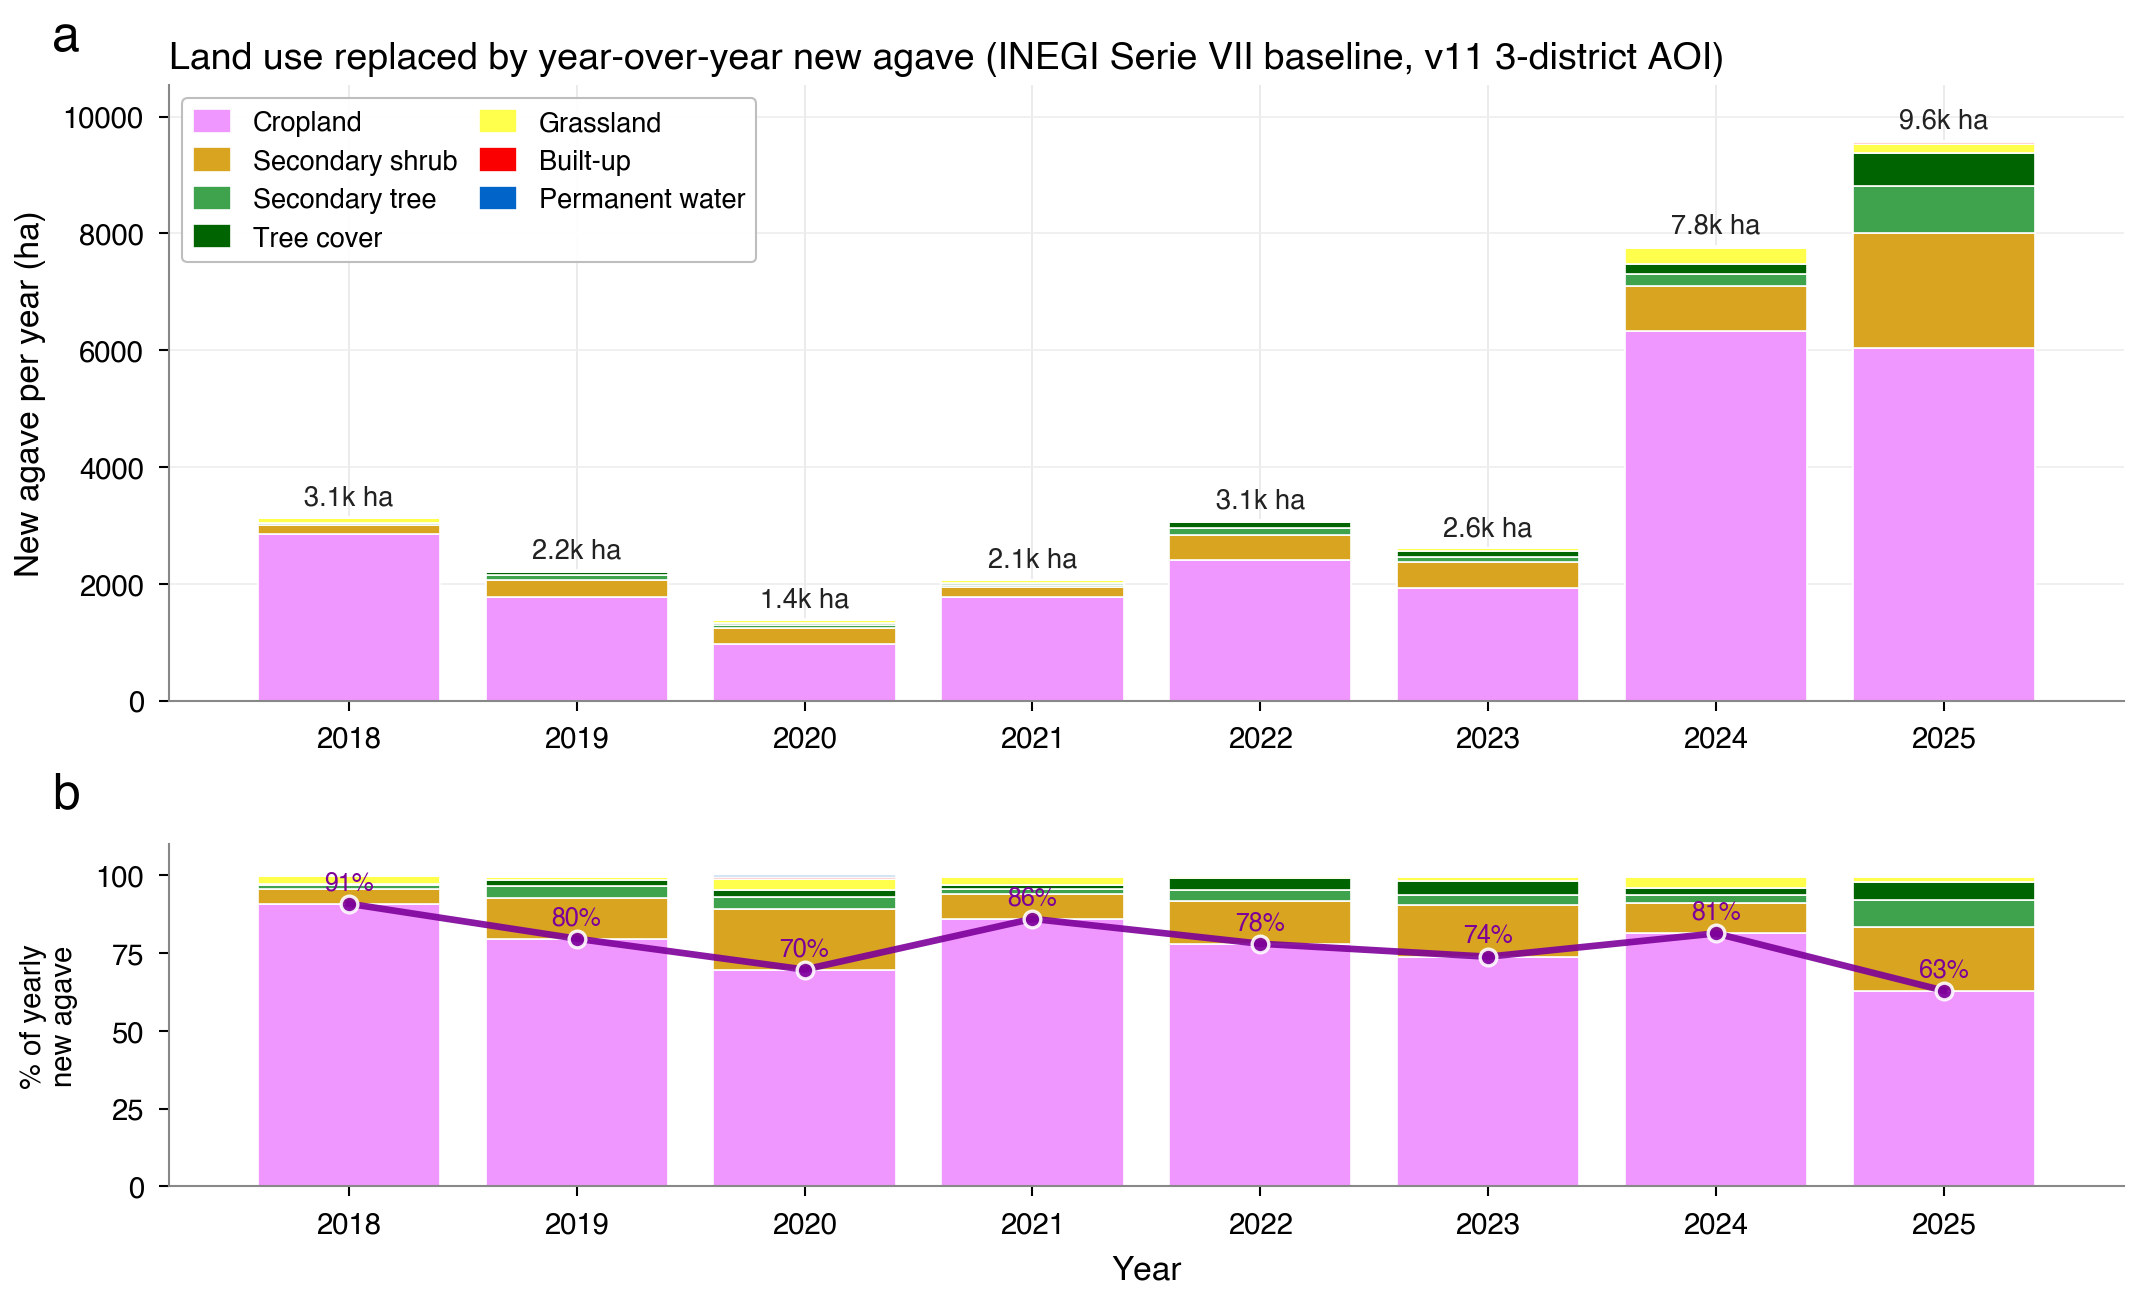
\includegraphics[width=\linewidth]{figures/fig9_v11_replaced_per_year.png}
  \caption{Per-year land-use composition of the v11 new-agave
  footprint, 2017$\to$2018 through 2024$\to$2025, under INEGI
  Serie VII (2018). \textbf{Panel a}: stacked absolute hectarage
  per year; the 2023$\to$2024 ($\sim$7.8\,k ha) and
  2024$\to$2025 ($\sim$9.6\,k ha) transitions account for $\sim$80\%
  of the eight-year boom. \textbf{Panel b}: stacked percentage
  composition with the cropland-share line (purple) annotated.
  Cropland is the dominant origin every year, ranging from 63\%
  (2024$\to$2025) to 91\% (2017$\to$2018).}
  \label{fig:replaced-year}
\end{figure}

\subsection{Synthesis: where, who, and what is replaced}\label{sec:results-synthesis}

Read together, the three result strands converge on a coherent
spatial--administrative--ecological signature for the v11 boom.
Spatially (Fig.~\ref{fig:spatial}), the 2017 footprint is confined
to the Tlacolula productive core; the 2020 panel shows the
post-2018 stabilisation; the 2023 panel captures the pre-acceleration
plateau; and the 2025 panel resolves the dramatic outward propagation
into the Yautepec basin and the upper Miahuatlán Sierra Sur.
Administratively (Fig.~\ref{fig:transitions}), the per-district
decomposition (panel~d) attributes 74\% of the 2025 footprint in
\textbf{Tlacolula} to new agave -- the historical core still grew
substantially in absolute terms ($+$9{,}000~ha) -- while
\textbf{Yautepec} and \textbf{Miahuatlán} are essentially
\emph{de novo} plantation territory, with 98\% and 96\% of their
2025 footprints classified as new agave between 2017 and 2025.
Ecologically (Fig.~\ref{fig:replaced-overall}), the
authoritative INEGI Serie VII baseline shows that 68.1\% of the
new agave displaces \textbf{cropland} (predominantly
\textit{agricultura de temporal anual}, i.e.\ rain-fed
smallholder \textit{milpa}), 24.7\% replaces secondary vegetation
(shrub + tree) in active regeneration, and only 5.2\% comes at
the direct expense of primary tree cover; the ESA WorldCover
2020 lens (panel~b) maps the same pixels predominantly to
``bare/sparse vegetation'' (32.8\%), a discrepancy attributable
to ESA's global, spectrum-driven labelling that under-distinguishes
the seasonally dry \textit{milpa} system. Together these three
results identify the v11 boom as primarily a 2024--2025
acceleration of \textbf{cropland-substitution agave expansion}
that propagates outward from the Tlacolula core into two
previously low-baseline districts -- a pattern with concrete
implications for milpa-dependent food sovereignty in the three
mezcal districts that we develop further in
\S\ref{sec:discussion}.

% =============================================================================
\section{Discussion}\label{sec:discussion}

\subsection{Magnitude and pulse structure of the boom}

The headline finding is a 4.4-fold expansion of agave extent
across the three-district mezcal footprint between 2017 and 2025:
raw map area rose $+336\%$ from 4{,}289~ha to 18{,}694~ha, a net
gain of $\sim$14{,}400~ha; the commission-corrected estimator
(raw $\times$ precision~$0.853$) yields the same percentage with
correspondingly smaller absolute hectarage. The bulk of this
expansion occurs in the last two years of the panel: 2024 alone
delivers an unprecedented $+107\%$ year-on-year change (doubling
of agave area in twelve months), and 2025 adds a further $+49\%$.
Both the raw and commission-only totals far exceed the SIAP
\textit{cierre agr\'icola} producer-reported total, consistent with
both under-reporting in the certified-producer registry (which
captures only the active certified palenques) and the inclusion in
our binary mask of informal, semi-wild and silvopastoral agave
that is spectrally similar to managed plantation but excluded from
the SIAP universe.

The pulse structure is strongly non-monotonic. The 2017 baseline
is followed by a 2018 pulse ($+44\%$), a 2019--2020 contraction
(deepest interim dip at $-22\%$ in 2020), a 2021--2022 recovery
($+6\%, +30\%$), a 2023 stall ($-3\%$), and then the explosive
2024--2025 acceleration. The interim 2019--2020 decline is
consistent with the multi-year harvest-and-replant cycle of
\textit{Agave angustifolia} (espad\'in, typically 6--8 years from
planting to maturity): mature stands harvested for production are
temporarily absent from the spectral signal until replant canopy
re-emerges. The 2024--2025 spike likely reflects a combination of
(i) the maturation of canopies established in the 2018 expansion
pulse, (ii) large-scale new planting in response to sustained
post-2020 export growth, and (iii) the geographic broadening of
plantation activity beyond the historical Tlacolula core into
Yautepec and Miahuatlán. Our binary mask cannot disambiguate
planted-but-immature, mature, harvested-and-replanted, or
wild-and-semi-wild agave; a multi-class follow-up with
species-level reference data is needed to confirm the mechanism.

\subsection{Spatial signature across the three districts}

Beyond aggregate totals, the per-district decomposition
(Fig.~\ref{fig:transitions}, panel d) shows that the 2024--2025
acceleration is not confined to the historical Tlacolula core.
Tlacolula remains the largest contributor in absolute terms, but
the new-agave fractional gain is highest in Miahuatlán and
Yautepec -- districts that started from a smaller 2017 baseline.
This spatial broadening is consistent with the hypothesis that
mezcal-driven plantation has saturated parts of the Tlacolula
productive belt (especially Santiago Matatlán and Tlacolula de
Matamoros) and is now propagating onto previously marginal land
in the upper Miahuatlán Sierra Sur (San Juan Ozolotepec, San
Mateo Río Hondo) and across the Yautepec basin (San Carlos
Yautepec, Santa María Ecatepec). A multi-class follow-up that
distinguishes \textit{A.\ angustifolia} from regional landraces
(\textit{A.\ marmorata}, \textit{A.\ karwinskii}) will be needed
to confirm whether the regional expansion reflects monoculture
espad\'in plantation or a more diverse, species-rich planting
front.

\subsection{Environmental footprint of the boom}

Under the authoritative INEGI Serie VII baseline
(\S\ref{sec:replaced}, Fig.~\ref{fig:replaced-overall}a), the
dominant transition pathway is \textbf{cropland substitution}:
\textbf{68.1\% of all new agave (10{,}492~ha) replaces existing
cultivated land}, predominantly rain-fed annual agriculture
(\textit{agricultura de temporal anual}) and irrigated annual
cultivation (\textit{agricultura de riego anual}). This is the
single most policy-relevant finding of the analysis. The mezcal
boom in the three core districts is overwhelmingly displacing
the \textit{milpa} (maize--bean--squash) system, fruit-orchards
and other smallholder food-production landscapes that anchor
rural food sovereignty in Oaxaca. The implications are concrete:
every hectare of agave added on this pathway corresponds to one
hectare of food-producing land withdrawn from local subsistence
and market supply, with downstream effects on milpa-dependent
species (\textit{Phaseolus} landraces, \textit{Cucurbita}
varieties), local maize prices and smallholder labour absorption.
Cropland substitution dominates every single year of the panel
(91\% in the 2017$\to$2018 pulse, 63\% in the 2024$\to$2025
pulse, $\sim$78\% on average).

A second, smaller but still meaningful pathway is conversion of
\textbf{secondary vegetation} -- 18.1\% from secondary shrub
(\textit{vegetaci\'on secundaria arbustiva}) plus 6.6\% from
secondary tree cover -- which represents land cleared at some
prior date (predating the 2018 INEGI baseline) and now in
shrub-arborescent regrowth. Re-clearance of recovering
vegetation forecloses ecological succession and reduces the
landscape's secondary-forest carbon sequestration potential,
although the impact is less acute than primary-forest loss.

Direct \textbf{primary-forest replacement} (\textit{bosque} and
\textit{selva}) is the most policy-sensitive category but only
the fourth-largest in absolute terms: \textbf{5.2\% of the boom
(806~ha across 2017--2025)}, concentrated along the upper
Miahuatlán Sierra Sur escarpment and the Yautepec basin edges.
The 2024$\to$2025 transition shows a modest uptick in the
combined primary + secondary tree share ($\sim$14\%) consistent
with the geographic broadening of the late-window expansion
pulses into previously forested terrain. The hectarage is
non-trivial and warrants targeted monitoring -- particularly
because primary \textit{bosque de encino} and \textit{selva baja
caducifolia} both occur in the affected munis -- but it does not
constitute the boom's dominant ecological footprint.

Together these findings shift the policy implications: the
mezcal Denomination of Origin should monitor not only
forest-edge expansion (a real but small fraction in absolute
hectares) but also, and primarily, the much larger ongoing
displacement of smallholder cropland and the re-clearance of
secondary vegetation in active regeneration. The
\textbf{disagreement between INEGI and ESA} on the dominant
substituted class (cropland vs bare/sparse) is itself a
substantive observation: global LC products defined by spectral
appearance miss the agronomic and cultural reality of dry-season
rain-fed cultivation in southern Mexico. Future remote-sensing
studies of agricultural boom commodities in similar contexts
should pair a global LC layer with a country-specific land-use
reference whenever one is available.

\subsection{Methodological observations}

The combination of AlphaEarth embeddings and a five-band terrain stack
proved sufficient to achieve $\kappa = 0.8018$ on this task at the
data-driven decision threshold without any custom spectral feature
engineering. AlphaEarth bands AE\_54, AE\_34 and AE\_03 carry the
largest mean-decrease-in-impurity contributions among the spectral
predictors; among terrain predictors, elevation contributes the most
signal, plausibly because the lower Tlacolula piedmont and the
upper Miahuatlán uplands differ in agave land-use intensity at
otherwise spectrally ambiguous scales.

The decision-threshold sweep underlying $\hat{\tau} = 0.60$ (see
\texttt{tools/threshold\_sweep.py}) is robust: seven of nine years
prefer an F1-optimal threshold in $[0.55, 0.75]$, and only 2017 and
2021 favour values outside that band (where the per-year positive
count is too low to trust the optimum). The global F1 optimum at
$\hat{\tau} = 0.60$ shifts the model from a precision-conservative
regime to a balanced F1 optimum (precision 0.853, recall 0.821, F1
0.837), which is appropriate for an inventory-style use case where
both omission and commission costs are roughly symmetric.

\subsection{Limitations}\label{sec:limitations}

Four limitations constrain interpretation. First, the
three-district AOI covers the Tlacolula, Yautepec and Miahuatlán
districts; it excludes other Oaxaca districts that contribute a
smaller share of statewide production (e.g.\ Ejutla, Sola de Vega,
Pochutla), and entirely excludes mezcal production outside Oaxaca
(Guerrero, Puebla, San Luis Potos\'i) which is small but rising.
Second, the 4{,}849-point reference panel concentrates in
Tlacolula (76\%) and Miahuatlán (23\%), with only $\sim$1\% of
polygons in Yautepec; the Yautepec area estimate may therefore
carry larger systematic error than the other two districts, and a
district-stratified panel extension is the highest-priority
next step. Third, the panel emphasises mature espad\'in
plantation; semi-wild populations of \textit{A.\ potatorum},
\textit{A.\ marmorata}, \textit{A.\ karwinskii}, and other
landrace species (which are particularly prevalent in Miahuatlán
and Yautepec) are mapped as a single \texttt{agave\_mature}
class, so species discrimination requires a multi-class extension.
Fourth, post-harvest stubble during the 6--18 months between
cutting and visible replant emergence is misclassified as
not-agave; a temporal hidden Markov post-processing pass would
smooth this artefact.

\subsection{Implications for governance}

The Consejo Regulador del Mezcal padr\'on currently captures a small
fraction of de facto plantation extent. The methodology described here
is sufficiently accurate, reproducible and inexpensive to deploy as a
standing surveillance tool for the Denomination of Origin, including
year-on-year monitoring of expansion onto slopes and into previously
forested cover types. Integration with the SIAP statistical universe
would clarify the magnitude of informal-sector production and reduce
asymmetries in the supply chain.

% =============================================================================
\section{Conclusions}\label{sec:conclusions}

Across the three core mezcal-producing districts of Oaxaca
(Tlacolula, Yautepec and Miahuatlán; 69 municipios,
$\sim$11{,}850~km$^2$), agave extent grew from 4{,}289~ha in 2017
to 18{,}694~ha in 2025 (a \textbf{4.4-fold increase, +336\% on raw
map area}; commission-corrected
3{,}658$\rightarrow$15{,}946~ha, also $+336\%$). The expansion was
strongly non-monotonic: an initial 2018 pulse ($+44\%$) was
followed by a 2019--2020 contraction (interim low at $-22\%$ in
2020 attributable to the espad\'in harvest cycle), modest recovery
through 2022, a 2023 stall, and then an unprecedented 2024
expansion of \textbf{$+107\%$} (agave area doubling in twelve
months) and a further $+49\%$ in 2025. The bulk of the absolute
hectare gain occurs in the final two years and propagates spatially
from the historical Tlacolula productive core into the Yautepec
basin and the upper Miahuatlán Sierra Sur. A histogram-based
gradient-boosting classifier on AlphaEarth Foundations annual
embeddings and a five-band terrain stack achieves overall accuracy
0.9425 and Cohen's $\kappa = 0.8018$ on an independent 870-point
test set at the data-driven decision threshold $\hat{\tau} = 0.60$.
The methodology is fully open and runs on free public
infrastructure, making it directly transferable to ongoing
monitoring of the Denomination of Origin and to other emerging
boom commodities.

\section*{Data and code availability}

All source code, GitHub Actions workflows, reference panels, and a
live interactive dashboard are available at
\href{https://github.com/iortiz1891/agave-boom-oaxaca}{github.com/iortiz1891/agave-boom-oaxaca}.
Reproducing the analysis end-to-end requires a Google Cloud Storage
bucket with the AlphaEarth and Copernicus DEM stacks and a free
GitHub Actions runner; the total compute footprint is approximately
3 runner-hours per model generation.

\section*{Acknowledgments}

We thank the Consejo Regulador del Mezcal for the palenque registry;
Google for releasing the AlphaEarth Foundations collection under the
Earth Engine catalogue; INEGI for the Marco Geoestad\'istico, the
\textit{Conjunto de Datos Vectoriales de Uso del Suelo y Vegetaci\'on}
Series, and the SIAP cierre agr\'icola; the Copernicus programme for
GLO-30; and the GitHub Actions free tier on which all compute was
performed. Errors are the author's own.

\bibliography{bibliography/refs}
\end{document}
